\section{Details of composition for
  glueing}\label{appendix:composition-glueing}

We build the element~$\Gamma \der b_1 = \comp^i~B~[\psi\mapsto
b]~b_0:(\Glue~[\varphi\mapsto(T,\myeq{})]~A)(i1)$ as the element
$\glue~[\varphi(i1) \mapsto t_1]~a_1$ where
%
\begin{align*}
  \Gamma,\varphi(i1) \der & \; t_1 : T(i1)[\psi \mapsto b(i1)]\\
  \Gamma \der & \; a_1 : A(i1)[\varphi(i1) \mapsto \myeq{}(i1) \; t_1,\psi \mapsto (\ugl~b)(i1)]
\end{align*}

As intermediate steps, we gradually build elements that satisfy more
and more of the equations that the final elements $t_1$ and $a_1$
should satisfy. The construction of these is given in five steps.

Before explaining how we can define them and why they are well
defined, we illustrate the construction in \fig{fig:compglue},
with $\psi = (j=1)$ and $\varphi = (i=0) \vee (j=1)\vee (i=1)$.

We pose $\delta = \forall i.\varphi$ (cf.\ \sect{sec:pathtypes}), so
that we have that~$\delta$ is independent from~$i$, and in our example
$\delta = (j = 1)$ and it represents the right-hand side of the
picture.
\begin{enumerate}
\item The element $a'_1:A(i1)$ is a first approximation of~$a_1$, but
  $a'_1$ is not necessarily in the image of~$\myeq{}(i1)$
  in~$\Gamma,\varphi(i1)$;
\item the partial element $\inctxt{\delta}{t'_1:T(i1)}$, which is a
  partial final result for~$\inctxt{\varphi(i1)}{t_1}$;
\item the partial path $\inctxt{\delta}{\omega}$, between~$a'_1$ and
  the image of~$t'_1$;
\item both the final element $\inctxt{\varphi(i1)}{t_1}$ and a path
  $\inctxt{\varphi(i1)}{\alpha}$ between~$a'_1$ and
  $\myeq{}(i1) \; t_1$;
\item finally, we build $a_1$ from~$a'_1$ and~$\alpha$.
\end{enumerate}
%
\begin{figure}[!h]
  \centering
  $$
\begin{tikzpicture}
  \coordinate (A00) at (0,0);
  \coordinate (A10) at ++ (3,0) ;
  \coordinate (A'11) at ++ (3,2) ;
  \coordinate (A'01) at ++ (0,2) ;
  \coordinate (A01) at ($(A'01) + (0,1.5)$);
  \coordinate (A11) at ($(A'11) + (0,1.5)$);

  \coordinate (O) at ($(A00) + (-4,1)$);
  \draw[fun line] (O) -- node[left] () {$i$} ++(0,1);
  \draw[fun line] (O) -- node[below] () {$j$} ++(1,0);

  % inner
  \begin{pgfonlayer}{background}
    \draw [path line] (A00) -- node [above] (a_0) {$\ugl~b_0$}
    (A10) -- coordinate (aj1)
    (A'11) -- coordinate (midA') (A'01);
    \draw [path line] (A01) -- coordinate (midA)
    node[above] () {Step 5: $a_1$} (A11);
    \draw (midA') node[below] {Step 1: $a'_1$} (A'01);
  \end{pgfonlayer}
  \draw (aj1) node[right, fill=white] () {$(\ugl~b)(j1)$};

  % links
  \begin{pgfonlayer}{background}
    \draw [fun line, <-] (A00) --
    node[left, xshift=-5] (f00) {$f$} ++ (-1,-1) coordinate (T00);
    \draw [fun line, <-] (A01) --
    node[left, xshift=-5] (f00) {$f$} ++ (-1,1) coordinate (T01);
    \draw [fun line, <-] (A10) --
    node[left, xshift=-5] (f00) {$f$} ++ (1,-1) coordinate (T10);
    \draw [fun line, <-] (A11) --
    node[left, xshift=-5] (f00) {$f$} ++ (1,1) coordinate (T11);
  \end{pgfonlayer}

  \fill (T11) circle [radius=2pt] node [right,xshift=10] () {Step 2:
    $\inctxt{\delta}{t'_1}$};

  \fill (A11) circle [radius=2pt] node [right,xshift=10,fill=white] ()
  {$\inctxt{\delta}{\myeq{}(i1) \; t'_1}$};

  % outer
  \begin{pgfonlayer}{background}
    \draw [path line] (T00) -- node[below] (b_0)
    {$\inctxt{\varphi(i0)}{b_0}$}
    (T10) -- coordinate (bj1)
    (T11) -- node[above] (t_1) {Step 4: $\inctxt{\varphi(i1)}{t_1}$} (T01);
    \draw [fun line] (b_0) -- node[left] {$\myeq{}$} (a_0);
  \end{pgfonlayer}
  \draw (bj1) node[right, fill=white] () {$b(j1)$};

  \draw [comp line] (A'11) -- node[right, xshift=10,fill=white] ()
  {Step 3: $\inctxt{\delta}{\omega}$ constant on $\psi$} (A11);

  % inner top diag edge
  % \coordinate (A''01) at ($(A'01) !0.25! (A01)$);
  % \draw [path line] (A''01) -- coordinate (midA'')
  %   node[below,yshift=-5] () {Step 4: $a''_1$} (A11);
  \draw [comp line] (midA') --
  node[left] () {Step 4': $\inctxt{\varphi(i1)}{\alpha}$} (midA);

\end{tikzpicture}
$$
\caption{Composition for glueing}
\label{fig:compglue}
\end{figure}

We define:
\begin{align*}
%  \Gamma,i:\II,\psi,\varphi\der t : T\label{eq:glue-t}\\
%  \Gamma,i:\II,\psi\der a = & \; \ugl~ b: A[\varphi\mapsto \myeq{} \;  b]%\label{eq:glue-a}
   \Gamma,\psi,i:\II \der a = & \; \ugl~ b: A[\varphi\mapsto \myeq{} \;  b]%\label{eq:glue-a}
  \\
%  \Gamma,\varphi(i0)\der t_0 : T(i0)[\psi\mapsto t(i0)]\label{eq:glue-t0}\\
  \Gamma\der a_0 = & \; \ugl~ b_0: A(i0)[\varphi(i0)\mapsto \myeq{}(i0) \; b_0,\psi\mapsto a(i0)]%\label{eq:glue-a0}
\end{align*}

\subparagraph*{Step 1} We define~$a'_1$ as the composition of~$a$
and~$\ugl~b_0$, in the direction~$i$, which is well defined since
$\ugl~b_0 = (\ugl~b)(i0)$ over the extent $\psi$
%
\begin{equation}
  \label{eq:glue-a'1}
  \Gamma \der a_1' = \comp^i~A~[\psi\mapsto~a]~a_0:A(i1)[\psi\mapsto~a(i1)]
\end{equation}
%\[\textrm{which is well defined because}\quad
%\begin{cases}
%  \Gamma,i:\II,\psi\der a : A \hfill \textrm{by~(\ref{eq:glue-a})}\\
%  \Gamma\der a_0 : A(i0)[\psi\mapsto a(i0)] \hspace{1cm} \textrm{by~(\ref{eq:glue-a0})}
%\end{cases}\]

\subparagraph*{Step 2} We also define~$t'_1$ as the composition of~$b$
and~$b_0$, in the direction~$i$:
%
\begin{equation}
  \label{eq:glue-t'1}
  \Gamma,\delta\der t_1' = \comp^i~T~[\psi\mapsto~b]~b_0:T(i1)[\psi\mapsto~b(i1)]
\end{equation}
\[\textrm{which is well defined because}\quad
\begin{cases}
  \Gamma,\delta,i:\II,\psi\der b : T \hfill
   \textrm{by Lemma \ref{admissible}} \\
  \Gamma,\delta\der b_0 : T(i0)[\psi\mapsto b(i0)] \hspace{1cm} \textrm{as~%(\ref{eq:glue-t0}) and
    $\delta \leqslant \varphi(i0)$}
\end{cases}\]
%
Moreover, since
\[
\begin{cases}
  \Gamma,\delta,\psi,i:\II \der a = \myeq{} \; b \hspace{1cm} \textrm{by~%(\ref{eq:glue-a}) and
    $\delta \leqslant \varphi$ ~~~~} \\
  \Gamma,\delta\der~a_0=\myeq{}(i0)~b_0 \hfill \textrm{by~%(\ref{eq:glue-a0}) and
    $\delta \leqslant \varphi(i0)$}
\end{cases}\]
we can re-express~$a'_1$ on the extent $\delta$
%
\[
\Gamma, \delta \der a_1' = \comp^i~A~[\psi\mapsto\myeq{}~b]~\left(\myeq{}(i0)~b_0\right)
\]
%
%Hence, the element~$a'_1$ restricted to the extent $\delta$ is the composition of images by~$\myeq{}$.

\subparagraph*{Step 3} We can hence find a path~$\omega$
connecting~$a'_1$ and~$\myeq{}(i1) \; t'_1$ in~$\Gamma,\delta$
using Lemma~\ref{pres}:
%
\[
\Gamma,\delta \der \omega = \pres{i}~\myeq{}~[\psi\mapsto b]~b_0 :
\left(\Path~A(i1)~a_1'~\left(\myeq{}(i1) \;
    t'_1\right)\right)[\psi\mapsto\pabs{j} a(i1)]
\]
%
Picking a fresh name~$j$, we have
%
\begin{equation}
  \Gamma,\delta,j:\II\der \omega~j : A(i1)[(j=0)\mapsto
  a'_1,(j=1)\mapsto \myeq{}(i1) \; t'_1,\psi\mapsto a(i1)]\label{eq:glue-omega}
\end{equation}

% \subparagraph*{Step 4} We then define~$a''_1$ as the composition
% of~$[\delta \mapsto \omega \; j, \psi \mapsto a(i1)]$ and~$a'_1$, in
% the direction~$j$:
% %
% \[\Gamma\der a''_1 = \comp^j~A(i1)~[\delta\mapsto \omega \; j,~\psi\mapsto
% a(i1)]~a_1' : A(i1)[\delta\mapsto\omega \; 1, \psi\mapsto a(i1)]
% \]
% \[\textrm{which is well defined because}\quad
% \begin{cases}
%   \Gamma,j:\II,\delta,\psi\der \omega~j = a(i1)
%   \hfill \textrm{by~(\ref{eq:glue-omega})} \\
%   \Gamma,j:\II,\delta\der \omega~0 = a'_1
%   \hfill \textrm{by~(\ref{eq:glue-omega})} \\
%   \Gamma,j:\II,\psi\der a(i1) = a'_1
%   \hspace{1cm} \textrm{by~(\ref{eq:glue-a'1})}
% \end{cases}
% \]
% and since $\Gamma,\delta\der\omega~1 = \myeq{}(i1) \; t'_1$,
% because~$\omega$ is a partial path between $a'_1$ and
% $\myeq{}(i1) \; t'_1$, we can re-express the type of~$a''_1$ in the
% following way:
% %
% \begin{equation}
% \Gamma\der a''_1 : A(i1)[\delta\mapsto\myeq{}(i1) \; t'_1,~\psi\mapsto a(i1)]\label{eq:glue-a''1}
% \end{equation}

\subparagraph*{Step 4} Now we define the final element~$t_1$ as the
inverse image of~$a'_1$ by~$\myeq{}(i1)$, together with the
path~$\alpha$ between~$a'_1$ and~$\myeq{}(i1) \; t_1$, in
$\Gamma,\varphi(i1)\der$, using Lemma~\ref{equiv}:
%
\[\Gamma,\varphi(i1)\der(t_1,\alpha) =
\eq~\myeq{}(i1)~[\delta\mapsto~(t'_1,\omega),\psi\mapsto~\left(b(i1),\pabs{j}a'_1\right)]~a_1'\]
\[{\textrm{with}\quad}\begin{cases}
  \Gamma,\varphi(i1)\der t_1 :
  T(i1)[\delta\mapsto~t'_1,\psi\mapsto~b(i1)] % \label{eq:glue-t1}
  \\
  \Gamma,\varphi(i1)\der\alpha :
  \left(\Path~A(i1)~a'_1~\left(\myeq{}(i1) \; t_1\right)\right)
  [\delta\mapsto\omega,\psi\mapsto~\pabs{j} a'_1)]
\end{cases}
\]
These are well defined because the two systems in~$\delta$ and~$\psi$
are compatible:
\[\begin{cases}
  \Gamma, \delta, \psi \der t'_1 = b(i1) & \textrm{by~(\ref{eq:glue-t'1})} \\
  \Gamma, \delta, \psi \der \omega = \pabs{j}a'_1 &
  \textrm{by~(\ref{eq:glue-omega}) and~(\ref{eq:glue-a'1})}
\end{cases}
\]
% %
% \[\begin{cases}
%   \Gamma,\varphi(i1),\delta\der a'_1 = \myeq{}(i1) \; t'_1
%   \hfill \textrm{by~(\ref{eq:delta-a'1})} \\
%   \Gamma,\varphi(i1),\psi\der a'_1 = a(i1) = \myeq{}(i1) \; b(i1)
%   \hspace{1cm} \textrm{by~(\ref{eq:glue-a'1}) in~$\Gamma,\psi\der$} %and~(\ref{eq:glue-a}) in~$\Gamma,\varphi\der$}
% \end{cases}\]
%
Picking a fresh name~$j$, we have
%
\begin{equation}
\Gamma,\varphi(i1),j:\II\der \alpha~j : A(i1)[(j=0)\mapsto
  a'_1,~(j=1)\mapsto \myeq{}(i1) \; t_1,~\delta\mapsto~a'_1,~\psi\mapsto a(i1)]\label{eq:glue-alpha}
\end{equation}

\subparagraph*{Step 5} Finally, we define~$a_1$ by composition
of~$\alpha$ and~$a'_1$:
%
\[\Gamma\der~a_1:=\comp^j~A(i1)~[\varphi(i1)\mapsto\alpha~j,\psi\mapsto~a(i1)]~a'_1:
A(i1)[\varphi(i1)\mapsto\alpha~1,\psi\mapsto~a(i1)]\]
\[\textrm{which is well defined because}\quad
\begin{cases}
  \Gamma,j:\II,\varphi(i1),\psi \der \alpha~j = a(i1)
  &\textrm{by~(\ref{eq:glue-alpha})} \\
  \Gamma,\varphi(i1)\der \alpha~0 = a'_1
  &\textrm{by~(\ref{eq:glue-alpha})} \\
  \Gamma,\psi\der a(i1) = a'_1
  &\textrm{by~(\ref{eq:glue-a'1})}
\end{cases}
\]
and since $\Gamma,\varphi(i1)\der\alpha~1 = \myeq{}(i1) \; t_1$, we can
re-express the type of~$a_1$ in the following way:
\[
  \Gamma\der a_1 : A(i1)[\varphi(i1)\mapsto\myeq{}(i1) \;
  t_1,~\psi\mapsto a(i1)]
\]
Which is exactly what we needed to build
$\Gamma\der b_1 := \glue ~[\varphi(i1)\mapsto t_1]~a_1:
B(i1)[\psi\mapsto b(i1)]$.

\medskip

\noindent Finally we check that $b_1 = \comp^i~T~ [\psi\mapsto~b]~b_0$
on $\delta$:
%
\begin{align*}
  b_1  &= \glue ~[\varphi(i1)\mapsto t_1]~a_1 &&\textrm{by def.} \\
  &=t_1 : T(i1)[\delta\mapsto~t'_1,\psi\mapsto~b(i1)]
  && \textrm{as $\varphi(i1) = 1_\FF$} \\
  &=t'_1 && \textrm{as $\delta = 1_\FF$} \\
  &= \comp^i~T~[\psi\mapsto~b]~b_0 &&  \textrm{by def.}
\end{align*}
% \[\begin{array}{llll}
% b_1  & = & \glue ~[\varphi(i1)\mapsto t_1]~a_1 & \hspace{2cm} \textrm{by def.} \\
%      & = & t_1 : T(i1)[\delta\mapsto~t'_1,\psi\mapsto~t(i1)] &
%      \hspace{2cm} \textrm{as $\varphi(i1) = 1_\FF$} \\
%      & = & t'_1 & \hspace{2cm} \textrm{as $\delta = 1_\FF$} \\
%      & = & \comp^i~T~[\psi\mapsto~b]~b_0 & \hspace{2cm} \textrm{by def.}
% \end{array}\]


\section{Univalence from glueing}
\label{sec:univ-from-glue}

We also give two alternative proofs of the univalence axiom for
$\Path$ only involving the glue construction.%
\footnote{The proofs of the univalence axiom have all been formally
  verified inside the system using the \Haskell{} implementation. We
  note that the proof of Theorem~\ref{thm:unglueequiv} can be given
  such that it extends $\myeq{}.2$ and hence in
  Corollary~\ref{cor:equiv-contr} we do not need the fact that
  $\isEquiv~X~A~\myeq{}.1$ is a proposition. For details see:\\
  \url{https://github.com/mortberg/cubicaltt/blob/v1.0/examples/univalence.ctt}}
The first is a direct proof of the standard formulation of the
univalence axiom while the second goes through an alternative
formulation as in Corollary~\ref{cor:equiv-contr}.%
\footnote{The second of these proofs is inspired by a proof by Dan Licata from:\\
  \url{https://groups.google.com/d/msg/homotopytypetheory/j2KBIvDw53s/YTDK4D0NFQAJ}}

\begin{lemma}
  \label{lem:ua-prel}
  For $\Gamma \vdash A : \U$, $\Gamma \vdash B : \U$, and an
  equivalence $\Gamma \vdash \myeq : \Equiv~A~B$ we have the following
  constructions:
  \begin{enumerate}
  \item\label{item:uap1} $\Gamma \vdash \eqToPath \myeq :
    \Path\, \U\, A\, B$;
  \item\label{item:uap2} $\Gamma \vdash \Path \, (A \to B) \,
    (\transport^i (\eqToPath \myeq \, i))) \, \myeq.1$ is
    inhabited; and
  \item\label{item:uap3} if $\myeq = \eq^i (P \, i)$ for $\Gamma
    \vdash P : \Path \, \U\, A \, B$, then the following type is
    inhabited:
    \[
    \Gamma \vdash %
    \Path \, (\Path \, \U \, A \, B) \, (\eqToPath {(\eq^i (P \, i))})
    \, P
    \]
  \end{enumerate}
\end{lemma}
\begin{proof}
  For \eqref{item:uap1} we define
  \begin{align}
    \label{eq:def-eqToPath}
    \eqToPath \myeq = \pabs i {\Glue \, [ (i=0) \mapsto
      (A,\myeq), (i=1) \mapsto (B, \eq^k B)] \, B }.
  \end{align}
  Note that here $\eq^k B$ is an equivalence between $B$ and $B$ (see
  \sect{subsec:compU}). For \eqref{item:uap2} we have to closely look
  at how the composition was defined for $\Glue$. By unfolding the
  definition, we see that the left-hand side of the equality is equal
  $\myeq.1$ composed with multiple transports in a constant type;
  using filling and functional extensionality, these transports can be
  shown to be equal to the identity; for details see the formal proof.

  The term for \eqref{item:uap3} is given by:
  \begin{align*}
    \pabs {j} \pabs {i} \Glue \,[ %
    &(i=0) \mapsto (A, \eq^k (P\, k)),\\
    &(i=1) \mapsto (B, \eq^k B),\\
    &(j=1) \mapsto (P \, i, \eq^k (P (i \lor k)))]\\
    &B \qedhere
  \end{align*}
\end{proof}

\begin{corollary}[Univalence axiom]
  \label{cor:ua}
  For the canonical map
  \[
  \can : (A \, B : \U) \to \Path \,\U\,A\,B \to \Equiv~A~B
  \]
  we have that $\can \, A \, B$ is an equivalence for
  all $A : \U$ and $B : \U$.
\end{corollary}
\begin{proof}[Proof 1]
  Let us first show that the canonical map $\can$ is path equal to:
  \[
  \eq = \lambda A \, B : \U. \, \lambda P : \Path\,\U\,A\,B. \, \eq^i (P\, i)
  \]
  By function extensionality, it suffices to check this pointwise.
  Using path-induction, we may assume that $P$ is reflexivity.  In
  this case $\can\,A\,A\,\refl{A}$ is the identity equivalence by
  definition.  Because being an equivalence is a proposition, it thus
  suffices that the first component of $\eq^i A$ is propositionally
  equal to the identity.  By definition, this first component is given
  by transport (now in the constant type $A$) which is easily seen to
  be the identity using filling (see \sect{sec:kan-filling}).

  Thus it suffices to prove that $\eq\,A\,B$ is an equivalence.  To do
  so it is enough to give an inverse (see Theorems 4.2.3 and 4.2.6 of
  \cite{hott-book}). But $\eqToPath$ is a left inverse by
  Lemma~\ref{lem:ua-prel}~\eqref{item:uap3}, and a right inverse by
  Lemma~\ref{lem:ua-prel}~\eqref{item:uap2} using that being an
  equivalence is a proposition.
\end{proof}
%
\begin{proof}[Proof 2]
  Points~\eqref{item:uap1} and~\eqref{item:uap2} of
  Lemma~\ref{lem:ua-prel} imply that~$\Equiv~A~B$ is a retract
  of~$\Path \,\U\,A\,B$. Hence $(X : \U) \times \Equiv~A~X$ is a
  retract of $(X : \U) \times \Path\,\U\,A\,X$.  But $(X : \U) \times
  \Path\,\U\,A\,X$ is contractible, so $(X : \U) \times \Equiv~A~X$ is
  also contractible as a retract of a contractible type. As
  discussed in~\sect{sec:univalence-axiom} this is an alternative
  formulation of the univalence axiom and the rest of this proof
  follows as there.
\end{proof}

Note that the first proof uses all three of the points of
Lemma~\ref{lem:ua-prel} while the second proof only uses the first
two. As the second proof only uses the first two points it is possible
to prove it if point~\eqref{item:uap1} is defined as in
Example~\ref{exa:equivtopath} leading to a slightly simpler proof of
point~\eqref{item:uap2}.

\section{Singular cubical sets}\label{sec-singular}

Recall the functor $\CC \to \Top, I \mapsto [0,1]^I$ given
at~\eqref{eq:georeal} in \sect{sec:cubecat}. In particular, the face
maps $(ib) \colon I-i \to I$ (for $b=0_\II$ or $1_\II$) induce the
maps $(ib)\colon [0,1]^{I-i} \to [0, 1]^{I}$ by $i(ib)u = b$ and
$j(ib)u = ju$ if $j\neq i$ is in $I$.  If $\psi$ is in $\FF(I)$ and
$u$ in $[0,1]^I$, then $\psi u$ is a truth value.

We assume given a family of idempotent functions
$r_I:[0,1]^I\times [0,1]\rightarrow [0,1]^I\times [0,1]$ such that
\begin{enumerate}
\item $r_I(u,z) = (u,z)$ if{f} $\partial_I u = 1$ or $z = 0$, and
\item for any {\em strict} $f$ in ${\sf Hom}(I,J)$ we have
  $r_J(f\times\id)r_I = r_J(f\times\id)$.
\end{enumerate}

\medskip

Such a family can for instance be defined as in the following picture
(``retraction from above center''). If the center has coordinate
$(1/2,2)$, then $r_I(u,z) = r_I(u',z')$ is equivalent to $(2-z')
(-1+2u) = (2-z) (-1+2u')$.
$$
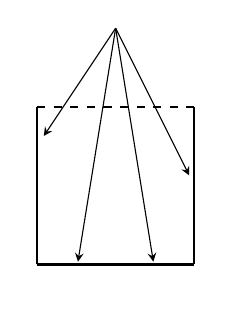
\begin{tikzpicture}[scale=2]
  % bottom
  \draw [thick,solid] (0,0) --
  node [near start,below=-1pt] (DL) {}
  node [near end,below=-1pt] (DR) {}
  (1,0);
  % left and right
  \draw [thick,solid] (0,0) --
  node [near end,](L) {} (0,1);
  \draw [thick,solid] (1,0) -- node (R) {} (1,1);
  % top
  \draw [dashed] (0,1) -- (1,1);
  % rays
  \def\raypt{(0.5,1.5)}
  \draw[->,>=stealth]\raypt -- (DL);
  \draw[->,>=stealth]\raypt -- (DR);
  \draw[->,>=stealth]\raypt -- (L);
  \draw[->,>=stealth]\raypt -- (R);
\end{tikzpicture}
$$

Property (1) holds for the retraction defined by this picture.
The property (2) can be reformulated as $r_I(u,z) =
r_I(u',z')\rightarrow r_J(f u,z) = r_J(f u',z')$. It also holds
in this case,
since $r_I(u,z) = r_I(u',z')$ is then equivalent to $(2-z') (-1+2u) = (2-z) (-1+2u')$,
which implies $(2-z') (-1+2f u) = (2-z)(-1+2 f u')$ if $f$ is strict.


Using this family, we can define for each $\psi$ in $\FF(I)$ an
idempotent function
\[
r_{\psi}:[0,1]^I\times [0,1]\rightarrow [0,1]^I\times [0,1]
\]
having for fixed-points the element $(u,z)$ such that $\psi u = 1$ or $z = 0$.
This function $r_{\psi}$ is completely characterized by the following properties:
\begin{enumerate}
\item $r_{\psi} = \id$ if $\psi = 1$
\item $r_{\psi} = r_{\psi}r_I$ if $\psi \neq 1$
\item $r_{\psi}(u,z) = (u,z)$ if $z = 0$
\item $r_{\psi}((ib)\times\id) = ((ib)\times\id)r_{\psi(ib)}$
\end{enumerate}

%% \medskip

%%  For instance, these functions witness the fact that the following polyhedrons, corresponding
%% respectively to the formula $\psi = ((i=1)\wedge (j=0))\vee (i=0)\vee (j=1)$
%% and $\psi = ((i=0)\vee (i=1))\wedge ((j=0)\vee (j=1))$, are retract of the
%% filled cube on directions $i,j,k$.

%% \[
%% \begin{tikzpicture}[scale=1.5, z=.5cm, rotate around y=5]
%%   % bottom
%%   \filldraw [thick,draw=black,fill=gray!30] (0,0,0) -- (1,0,0) -- (1,0,1) --
%%   (0,0,1) -- cycle;
%%   % back
%%   \filldraw [thick,draw=black,fill=gray!60] (0,0,1) -- (1,0,1) -- (1,1,1) --
%%   (0,1,1) -- cycle;
%%   % right
%%   \filldraw [thick,draw=black,fill=gray!60] (1,0,0) -- (1,1,0) -- (1,1,1) --
%%   (1,0,1) -- cycle;
%%   % pins
%%   \draw [thick, black] (0,0,0) -- (0,1,0);
%%   \draw [thick, black] (1,0,0) -- (1,1,0);
%%   % points
%%   \draw [thick, fill = black, circle] (0,0,0) circle (0.05);
%%   \draw [thick, fill = black, circle] (0,1,0) circle (0.05);
%% %  \node[align = center, below]{$\psi$ = (i=0)\vee (j=0)\vee ((i=1)\wedge (j=1))};
%% \end{tikzpicture}
%% \qquad\qquad
%% \begin{tikzpicture}[scale=1.5, z=.5cm, rotate around y=5]
%%   % bottom
%%   \filldraw [thick,draw=black,fill=gray!30] (0,0,0) -- (1,0,0) -- (1,0,1) --
%%   (0,0,1) -- cycle;
%%   % back
%%   \filldraw [thick,draw=black,fill=gray!60] (0,0,1) -- (1,0,1) -- (1,1,1) --
%%   (0,1,1) -- cycle;
%%   % left
%%   \filldraw [thick,draw=black,fill=gray!50] (0,0,1) --
%%   (0,1,1) -- (0,1,0) -- (0,0,0) -- cycle;
%%   % right
%%   \filldraw [thick,draw=black,fill=gray!80] (1,0,0) -- (1,0,1) --
%%   (1,1,1) -- (1,1,0) -- cycle;
%%   % back
%%   \filldraw [thick,draw=black,fill=gray!90] (0,0,0) -- (1,0,0) -- (1,1,0) --
%%   (0,1,0) -- cycle;
%%   % points
%% \end{tikzpicture}
%% \]

These properties imply for instance $r_{\partial_I}(u,z) = (u,z)$ if
$\partial_I u = 1$ or $z=0$ and so they imply $r_{\partial_I} = r_I$.
They also imply that $r_{\psi}(u,z) = (u,z)$ if $\psi u = 1$.

\medskip

From these properties, we can prove the uniformity of the family of
functions $r_{\psi}$.

\begin{theorem}
  If $f$ is in ${\sf Hom}(I,J)$ and $\psi$ is in $\FF(J)$, then
  $r_{\psi}(f\times\id) = (f\times\id)r_{\psi f}$.
\end{theorem}

This is proved  by induction on the number of element of $I$ (the
  result being clear if $I$ is empty).

A particular case is $r_J(f\times\id) = (f\times\id)r_{\partial_J
  f}$. Note that, in general, $\partial_Jf$ is not $\partial_I$.

\medskip

A direct consequence of the previous theorem is the following.

\begin{corollary} The singular cubical set associated to a topological space
has a composition structure.
\end{corollary}


%% Local Variables:
%% mode: latex
%% TeX-master: "main"
%% End:
